
% VLDB template version of 2020-08-03 enhances the ACM template, version 1.7.0:
% https://www.acm.org/publications/proceedings-template
% The ACM Latex guide provides further information about the ACM template

\documentclass[sigconf, nonacm]{acmart}
\usepackage{todonotes}
\usepackage{fancyhdr,graphicx,amsmath}
\usepackage[ruled,vlined]{algorithm2e}
\usepackage{algorithmic}
\usepackage{subfigure}
\usepackage{float}
\usepackage{stfloats }
\usepackage{csquotes }

\usepackage{multirow}



\usepackage[english]{babel}
\usepackage{blindtext,letltxmacro,xcolor,xparse}
\usepackage{lipsum}% for simulating real text

\LetLtxMacro{\blindtextblindtext}{\blindtext}
\LetLtxMacro{\blindtextBlindtext}{\Blindtext}

\RenewDocumentCommand{\blindtext}{O{\value{blindtext}}}{%
  \begingroup\color{gray}\blindtextblindtext[#1]\endgroup
}
\RenewDocumentCommand{\Blindtext}{O{\value{blindtext}}O{\value{Blindtext}}}{%
  \begingroup\color{gray}\blindtextBlindtext[#1][#2]\endgroup
}

\usepackage{amsmath}
\DeclareMathOperator{\foz}{foz}
\DeclareMathOperator{\val}{\textbf{val}}
\DeclareMathOperator{\hash}{\textbf{murmur3}}
\DeclareMathOperator{\get}{\textbf{get}}
\DeclareMathOperator{\insertv}{\textbf{insert}}


% Algorithmic modifications
\makeatletter
\newcommand{\ALOOP}[1]{\ALC@it\algorithmicloop\ #1%
  \begin{ALC@loop}}
\newcommand{\ENDALOOP}{\end{ALC@loop}\ALC@it\algorithmicendloop}
\renewcommand{\algorithmicrequire}{\textbf{Input:}}
\renewcommand{\algorithmicensure}{\textbf{Output:}}
\newcommand{\algorithmicbreak}{\textbf{break}}
\newcommand{\BREAK}{\STATE \algorithmicbreak}
\makeatother


\usepackage[nocfg]{nomencl}
\makenomenclature


%% The following content must be adapted for the final version
% paper-specific
\newcommand\vldbdoi{XX.XX/XXX.XX}
\newcommand\vldbpages{XXX-XXX}
% issue-specific
\newcommand\vldbvolume{14}
\newcommand\vldbissue{1}
\newcommand\vldbyear{2020}
% should be fine as it is
\newcommand\vldbauthors{\authors}
\newcommand\vldbtitle{\shorttitle}
% leave empty if no availability url should be set
\newcommand\vldbavailabilityurl{https://github.com/mlaass/counting-globimaps}
% whether page numbers should be shown or not, use 'plain' for review versions, 'empty' for camera ready
\newcommand\vldbpagestyle{plain}

\begin{document}
\title{Counting GloBiMaps - A Probabilistic Data Structure for Handling Big Point Datasets}

%%
%% The "author" command and its associated commands are used to define the authors and their affiliations.
\author{Moritz Laass}
\affiliation{%
  \institution{Technical University of Munich}
  \department{TUM School of Engineering and Design}
  \streetaddress{Lise-Meitner-Str. 9}
  \city{Munich}
  \state{Germany}
  \postcode{85521}
}
\email{moritz.laass@tum.de}

\author{Martin Werner}
\affiliation{%
  \institution{Technical University of Munich}
  \department{TUM School of Engineering and Design}
  \streetaddress{Lise-Meitner-Str. 9}
  \city{Munich}
  \state{Germany}
  \postcode{85521}
}
\email{martin.werner@tum.de}



%%
%% The abstract is a short summary of the work to be presented in the
%% article.
\begin{abstract}
  In this paper, we define a probabilistic data structure based on a layered construction built from Counting Bloom Filters and analyze the properties of this construction on real-world datasets. The key idea of the approach is to design a series of layers, each of which can accommodate a certain number of identical points. By taking a first layer to incorporate only small numbers, but for a comparably large number of different input values, the long tail of spatial data distributions can be well-served. Those slots of the first layer that are forced to overflow due to hash collisions or frequent items in the input distribution are transferred to a next layer of different characteristics. Multiple layers can be stacked and the spatial resolution can be modified to further increase the flexibility of the data structure. We show that basic Bloom filter operations such as the union and intersection can be lifted to this construction and show that the construction can be used to count data points in polygons or other complex geometries, without the need for unpacking. Case studies on map data from OpenStreetMap and social media data from Twitter illustrate the real-world behavior of this data structure.
\end{abstract}

\maketitle

%%% do not modify the following VLDB block %%
%%% VLDB block start %%%
\pagestyle{\vldbpagestyle}
\begingroup\small\noindent\raggedright\textbf{PVLDB Reference Format:}\\
\vldbauthors. \vldbtitle. PVLDB, \vldbvolume(\vldbissue): \vldbpages, \vldbyear.\\
\href{https://doi.org/\vldbdoi}{doi:\vldbdoi}
\endgroup
\begingroup
\renewcommand\thefootnote{}\footnote{\noindent
  This work is licensed under the Creative Commons BY-NC-ND 4.0 International License. Visit \url{https://creativecommons.org/licenses/by-nc-nd/4.0/} to view a copy of this license. For any use beyond those covered by this license, obtain permission by emailing \href{mailto:info@vldb.org}{info@vldb.org}. Copyright is held by the owner/author(s). Publication rights licensed to the VLDB Endowment. \\
  \raggedright Proceedings of the VLDB Endowment, Vol. \vldbvolume, No. \vldbissue\ %
  ISSN 2150-8097. \\
  \href{https://doi.org/\vldbdoi}{doi:\vldbdoi} \\
}\addtocounter{footnote}{-1}\endgroup
%%% VLDB block end %%%

%%% do not modify the following VLDB block %%
%%% VLDB block start %%%
\ifdefempty{\vldbavailabilityurl}{}{
  \vspace{.3cm}
  \begingroup\small\noindent\raggedright\textbf{PVLDB Artifact Availability:}\\
  The source code, data, and/or other artifacts have been made available at \url{\vldbavailabilityurl}.
  \endgroup
}
%%% VLDB block end %%%

\section{Introduction}
The management of large datasets has been a quite vibrant area of research in the last decades. Organizational schemes based on tree orderings of data spaces dominate the field (e.g., R-trees, ball trees) for their excellent performance and wide availability. However, it has also been realized that tree access methods have their limitations especially in parallel and distributed contexts. Locality sensitive hashing (LSH) and - in general - more random data distribution methods have taken the lead for data that is growing beyond a practicable size for consistent query execution. In this context, Bloom filters play a vital role both in the coordination of nodes as well as in the context of log merge trees and key value stores. In these, Bloom filters are widely used to quickly assess if a certain block of data (e.g., a sorted string table on disk, a node in a distributed system, etc.) contains information about a certain key.

In this context, Bloom filters have been used literally as filter algorithms: they provide a compressed representation of what there might be in a data block and can reduce irrelevant I/O operations significantly with a small memory overhead. In this scenario, Bloom filters are optimized to be extremely small and fast: each object shall be modeled with only few bits and only very few hash function computations.

In previous work, we have investigated if and how Bloom filters can be used to directly model interesting datasets going for configurations with up to 32 GB of memory assigned for a single Bloom filter. We used Bloom filter for modeling huge, but sufficiently sparse geospatial raster datasets \cite{werner2019globimaps, werner2021globimapsai} and trajectories of moving objects \cite{werner2015bacr}.

In this paper, we present a data structure Counting GloBiMap (CGM), which extends on classical GloBiMaps \cite{werner2019globimaps} by replacing
Bloom filters with Counting Bloom filters of varying bit depth. Due to the power law structure of typical datasets, the discretization inherent to
GloBiMaps leads to few objects with extremely high observation frequency in input data (e.g., locations with a high number of messages) and the majority of locations with moderate to small numbers of data items associated.

In order to deal with this data distribution, we first choose a small number of bits for the counting bloom filter, such that many of the involved bits will overflow during data intake. In this context, the data structure uses a multilayer approach. The data structure is configurable to hold as many layers as necessary, whereas each layer basically represents a counting Bloom filter with a fixed size and bit-depth and the insertion of a new element will increment the first non-maximal layer of the construction. That is, in the beginning, all insertions increment locations in the first filter. As soon as a few slots of the first layer reach their maximal value of an all-one bit string, the insertion is forwarded to the second layer.

This setup allows for a pyramid like construction of the multiple layers, with the lower layers being of bigger sized filters with lower bit-depth per slot, while the higher layers are comprised of smaller sized filters with higher bit-depth. While there have been approaches in Bloom Filters, that take the distribution of the to be contained data into account \cite{ficara_multilayer_2008} \cite{bruck2006weighted}. The way our data structure operates has not been proposed so far. Additionally, the simplicity of our approach also holds promise to enable a straight forward implementation even in reconfigurable devices and hardware \cite{cho2014fpga, ramachandran2015fpga, harwayne2009fpga}. In addition, we expect predictable performance, as bit-depths that are native to the hardware environment and fixed size filters will in most cases lead to better performance and memory layouts than some of the approaches in the literature, that rely on dynamic resizing of filters and bin sizes \cite{guo2009dynamic}.

%While we only give a C++ implementation for general purpose processors in this work, implementations for specialized hardware such as GPUs, FPGAs and ASICs seem feasible and straight forward, given the suggested data layout.

Another interesting fact about the data structure is the possibility of performing certain operations using the compressed representation without the need to unpack the data into a more classical representation, such as a bitmap or (sparse) matrix. We show that this property might be useful to approximate some types of spatial queries, for example counting points in a polygon. While the approximation of a query in such a probabilistic setting is interesting in itself, we envision additional help for query planning as these data structures give access to frequency information and expected candidate set or result set sizes as well. This could either be used to stop queries that contain a too large result set, or to decide about sub query priorities and distribution strategies, which has been successfully proposed using simple Bloom filters \cite{michael2007improving, lee2012join, papapetrou2010cardinality}.

The remainder of the paper is structured as follows: in Section \ref{related-work} we shortly review previous work related to our research. In Section \ref{counting-globimaps}, a thorough overview of the data structure and its properties is given. In Section \ref{operations-on-counting-globimaps}, a set of operations on Counting GloBiMaps is introduced, which can be used to model certain types of queries. In Section \ref{evaluation}, an experimental evaluation on real world spatial datasets is presented, documenting the behaviour and performance of our data structure. Section \ref{conclusion} concludes the paper.

%\nomenclature{$a$}{The number of angels per unit area}%
%\nomenclature{$N$}{The number of angels per needle point}%
%\nomenclature{$A$}{The area of the needle point}%
%%The equation $\sigma = m a$%
%\nomenclature{$\sigma$}{The total mass of angels per unit area}%
%\nomenclature{$m$}{The mass of one angel}
%
%\printnomenclature


\section{Related Work}\label{related-work}

In this section, we discuss Bloom filters  which have been invented to represent extremely sparse subsets of strings, such as English words with irregular spelling and have since been used in various applications. Further, we examine Counting Bloom filters which are an extension to Bloom filters allowing for a scalar representation of entries instead of a binary one.
Despite the fact that Bloom filters and Counting  Bloom filters have been frequently used in big data systems, it has not yet been applied to represent sparse frequency rasters. However standard Bloom filters have been used to represent small collections of locations in web browsers \cite{ruppel2014geocookie} as well as trajectories \cite{werner2015bacr} and geospatial bitmaps in the previous work on globimaps \cite{werner2019globimaps}

%\begin{comment}
%\subsubsection{Sparse Matrices}
%In a sparse matrix the majority of Values are zero. There is no clear specification of how many zero-value elements a matrix must have to be considered sparse, but one frequent requirement is that the number of non-zero elements must be roughly equal to the number of rows or columns. When the majority of the components are non-zero, the matrix is said to be dense.  In computing, a sparse matrix is one in which the set of non-zero entries is represented by tuples $(I j,v)$, where $I$ and $j $represent the row and column, respectively, and $v$ represents the value. Point clouds with integer coordinates can be used to identify sparse matrices, and all aspects of spatial indexing can be used to speed up access to sparse matrices' entries.
%
%Sparse matrices,  are commonly represented in one of two ways: as a naive form in which the tuples are sorted and structured as a dictionary or a list of lists, or as a form in which the tuples are ordered and organized as a list of lists or a collection of lists, or in a linear algebra-optimized format, such as compressed sparse row (CSR) and compressed sparse column (CSC) \cite{globimaps_2} . However, in addition to the data, all of these sparse matrices data structures hold two integer indices. One of these integer indices in CSR and CSC can be compressed to retain simply the beginning of each line, but the second index column is the same size as the number of non-zero elements. As a result, a sparse matrix usually requires at least $2n + m$ memory cells, where $n$ denotes the number of non-zero entries and $m$ denotes the number of rows (in CSR, in CSC columns respectively ).
%
%\subsubsection{Image File Formats}
%Image compression is a well-known issue that has received a lot of attention in the computer graphics and signal processing fields.
%
%The image formats given, on the other hand, are frequently based on assumptions that are incorrect for global raster data sets. Some of these file formats require that a file be utilized completely and that it be decoded in its entirety before being used. This is true, for example, for JPEG images and portable network graphics. Most implementations (such as libpng and libjpeg) load the entire image into main memory and make it accessible as a dense matrix. Nonetheless, these formats are commonly used in the context of global raster data sets, such as for distributing spatial data sets to consumers via the Internet. The de-facto norm for presenting large raster graphics on the web is still a web map service built on tiles of little 256x256 pixel pictures. The tagged image file format (TIFF) is another image file format that is suited for huge data sets and allows only parts of the image to be decoded \cite{globimaps_7} As a result, the image is divided into strips (for example, numerous consecutive scanlines) or tiles (for example, rectangular data chunks) that can be read separately. Because each access must load the entire strip or tile where the data sits, this architecture does not support real random lookups. However, the TIFF image file format is commonly used in Geographic Information Systems (GIS) since there is a defined extension known as GeoTIFF \cite{globimapm_10}, which contains information about the spatial projection of the picture data in the image file's header.
%In conclusion, storing a global raster data set as a collection of image files is a viable strategy for most application scenarios, but it incurs significant overhead if pixelwise random access occurs frequently, because a large environment of the pixel is decoded into main memory before answering the query for this pixel.
%\end{comment}
%

\subsection{Bloom Filters}

The Bloom filter data structure was introduced by Bloom in 1970. It is a probabilistic data structure capable of encoding sets in main memory \cite{bloom_space/time_1970}. It gives the option of deciding how much memory to utilize to model the set, trading memory consumption and compute effort with error probability. However, the most essential feature of Bloom filters is that they only have one type of errors: false positives. While the data structure representing a set will never forget an element that has been added to the set, it may report elements that have never been added to the set as belonging to the set. But this error can be kept arbitrary small by investing more computation and memory. The Bloom filter's basic structure is as follows:

One starts by defining $F$ as an $m$-bit array. We then use $k$ pairwise independent hash functions $h_i$ that map all of the set's potential elements to a non-negative integer value less than $m$. An all-zero Bloom filter array $F$ represents the empty set. The Bloom filter now has two operations: Insert and Test, which expose its capabilities. The function Insert alters the Bloom filter to express the fact that an element has been introduced, given an element $e$. Given the limitation of false positive findings, the function Test reports whether the data structure suggests that the element has been entered before. The value of the specified $k$ hash functions applied to the provided element $e$ is calculated first in both processes. The Insert function sets all of the slots designated by the hashing results to one, but the Test function indicates that the element is not in the set if one of these outcomes refers to a zero slot. The Insert operation sets the same bits to one that the Test function searches for a zero, therefore there can't be any false negatives in this data structure. When all of the slots indexed by hash functions are filled with ones, on the other hand, we can assume that the element has been entered, even though the values could have originated from a combination of adding distinct elements due to probable hash collisions. Note that the Insert operation will always compute all hash values and access all indexed locations while the Test operation is capable of early stopping on the first zero encountered.

It's fascinating to see how errors in this data structure can be modeled. A Bloom filter with $n$ elements can be viewed as the consequence of setting an essentially random bit in the underlying array to one for $kn$ times, with the hash functions transforming the elements into uniformly distributed random integers.
Finding a false positive is now as likely as finding $k$ ones in random filter slots, which is as likely as finding a one $k$ times in a random slot.
In fact, the following formula connects the parameters $m, k$, and the number of inserted elements $n$ to a fraction of zeros measure ($\foz$).

\begin{equation}
  \foz = \left(1- \frac{1}{m} \right) ^{k n} \approx e^{\frac{-k n}{m}}
\end{equation}

This fraction of zeros is a suitable proxy for the likelihood of discovering a zero in a random location assuming the hash functions are sufficiently random and independent (thus also assuming sufficiently large filters). As a result, the filter's false positive probability can be estimated as follows: If $k$ random accesses to the bit field discover a one, a false positive occurs.
\begin{equation}
  p = (1-\foz)^k \approx \left(1-  e^{\frac{-k n}{m}} \right)^k
\end{equation}

We may search for a minimum of $k$ by differentiating this equation and locating the roots because the right hand side is differentiable. This leads to the conclusion, that
\begin{equation}
  k_{*} = \frac{m}{n} \ln{2}
\end{equation}

is the (anticipated) false positive rate's global minimum. That is, we can determine an optimal value $k_{*}$ given a memory budget of $m$ bits and a number of components $n$ to be fed into the filter. However, because $k$ is required to be an integer number of hash functions, we will need to round $k_{*}$ to the nearest integer. Furthermore, $m$ is often constrained to memory pages or even powers of two to allow for faster modulo computation and the value of $n$ is rarely known beforehand \cite{broder2004network}.

%Notable when it comes to Counting Bloom Filters (see \ref{section:cbf}) is the fact that $n$ is the distinction between the number of elements inserted into the filter, and the number of uniquely positions entered into the filter. Depending on the distribution of the data the number of unique positions will be magnitudes smaller than the number of elements. Which means, that if the distribution of data is known more precise predictions of errors and their sizes can be made than what is discussed in the previous literature.


\subsection{Counting Bloom Filters}\label{section:cbf}
Many papers on BFs have been published, with compressed BFs \cite{mitzenmacher2002compressed}, distance-sensitive BFs \cite{kirsch2006distance} dynamic BFs \cite{guo2009dynamic}, being some of the most important innovations in the area of BFs.

As previously noted, BFs are strictly binary in the sense that they can only tell if an item is in the set or not, but not how many items of the same value have been added, nor do they allow for the removal of items from a set in a sensible way. Towards this end, Counting Bloom Filters (CBFs) were introduced by Fan in 2000 \cite{fan2000summary} which use small unsigned integer bins rather than single bits of presence. The appropriate bin counters are incremented when an item is inserted or decremented when removed.
While CBFs have many desirable properties, they introduce the issue of counter overflow, which must be considered when designing the data structure. Many enhancements to CBFs have been made in attempt to overcome these constraints and to gain improved performance. And the amount of main memory is now significantly higher, especially when common CPUs with a smallest adressable unit of 8 bits are used. It is very tricky to efficiently implement 3-bit counters on 64 bit CPUs.

DCFs (Dynamic Count Filters) \cite{aguilar-saborit_dynamic_2006} are basic data structures designed for speed of retrieval and adaptability. They do not require the usage of indexes like other schemes, thus resulting in fast access times and the ability to store arbitrary amounts of data.

DCFs are made up of two vectors: one is a standard CBF with fixed-size counters, and the other is an Overflow Counter Vector with a counter for each element of the first vector that keeps track of the number of overflow occurrences. To avoid saturation, the size of counters in overflow counter vector is changed dynamically.
This of course means that each update requires rebuilding of the data structure, which comes with a significant performance overhead for insertions, which is different from our approach.  Other schemes such as Multilayer Compressed Counting bloom filters are utilising Huffman codes to optimize bin size and have introduced the idea of a hierarchical multilayer structure \cite{ficara_multilayer_2008}.
% Stress difference between DCFs and our proposal. Maybe to stack multiple layers?

\subsubsection{Binary GloBiMaps}

In a previous paper Global Binary Maps (GloBiMaps) were introduced using binary Bloom filters to represent global raster data sets in the spatial domain. It was shown that many desirable properties of 2D raster datasets still hold true in this representation such as low resolution incremental rendering, the ability to form quadtrees using alternating coding, low memory overhead error correction and fast compression using the mod-2 strategy \cite{werner2019globimaps}.

For GloBiMaps, a global sparse raster (e.g., all human built-up area in the world) is used and the integer raster coordinates are hashed in order to write into a Bloom filter. An additional error correction table makes sure that false positives of the structure are corrected. Experiments show that extreme compression ratios are possible and common for certain sufficiently sparse datasets. Furthermore, the false positives have been interpreted as the addition of a uniform random noise to the underlying truth and we were able to remove a huge part of this noise by training a convolutional neural denoiser in residual representation \cite{werner2021globimapsai}. In this way, we were able to accommodate a higher amount compression ratios efficiently, but at the cost of of allowing false negatives introduced by the denoising scheme.

\section{Counting GloBiMaps}\label{counting-globimaps}

%\begin{comment}
%
%
%\begin{figure*}[b]
%  \def\pfw{.15\textwidth}
%  \centering
%  \subfigure[Bin Sizes at 2048 x 2048 Pixel Resolution]{    
\includegraphics[width=\pfw, page=1]{figures/histograms_Twitter 200 mio.pdf}}
%  \subfigure[Bin Sizes at 2048 x 2048 Pixel Resolution]{    
\includegraphics[width=\pfw, page=2]{figures/histograms_Twitter 200 mio.pdf}}
%  \subfigure[Bin Sizes at 8192 x 8192 Pixel Resolution]{    
\includegraphics[width=\pfw, page=5]{figures/histograms_Twitter 200 mio.pdf}}
%  \subfigure[Bin Sizes at 8192 x 8192 Pixel Resolution]{    
\includegraphics[width=\pfw, page=6]{figures/histograms_Twitter 200 mio.pdf}}
%  \subfigure[Bin Sizes at 16384 x 16384 Pixel Resolution]{    
\includegraphics[width=\pfw, page=7]{figures/histograms_Twitter 200 mio.pdf}}
%  \subfigure[Bin Sizes at 16384 x 16384 Pixel Resolution]{    
\includegraphics[width=\pfw, page=8]{figures/histograms_Twitter 200 mio.pdf}}
%
%  \caption{Histograms for First 200 mio Points of the Twitter Dataset}
%  \label{fig:hist_twitter}
%\end{figure*}
%\end{comment}
%

%Counting GloBiMaps (CGM) are an implementation of Counting Bloom Filters
%that adopt a simple but effective strategy to address the overflow
%problem caused by the limitation of the bit-depth for the standard CBF bins.


\begin{figure}[h!]
  \def\pfw{.45\textwidth}
  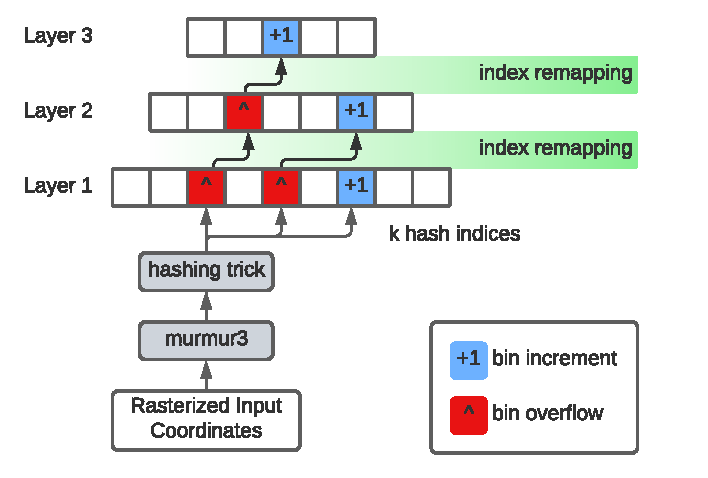
\includegraphics[width=\pfw, page=1]{figures/CGM_Layer_Schema.pdf}
  \caption{CGM MultiLayer Structure}
  \label{fig:cgm_schema}
\end{figure}

Figure \ref{fig:cgm_schema} depicts the construction of Counting GloBiMaps in the context of managing spatial point cloud datasets or frequency rasters. Similar to GloBiMaps, we start with spatial input data points such as messages or events. In a first step, we discretize the
coordinates of the spatial objects (e.g., we rasterize them) and apply a combination of a good and fast hash function (Murmur3 in our implementations) and the hashing trick  to generate values of $k$ sufficiently independent uniform hash values.
These hash values are now used to address an array of small counters as in the Counting Bloom filter construction descending into higher layers in case of overflow.

More precisely, a  Counting GloBiMaps consists of a set of $k$ hash function
and a set of $\Lambda$ layers $L_x$ each consisting of a filter of
size $m_x$ with bins of bit depth $b_x$.

$$CGM = \{k, L_x = \{m_x, b_x\} \} \space x=1..\Lambda  $$

For a bit-depth $b_x$, the threshold value $T_x$ is computed as

$$ T_x = 2^{b_x}-1$$

The bins of the first layer are incremented until they reach the threshold value
$T_1$. Then, the corresponding bin of the second layer is
incremented. This scheme is then repeated for subsequent layers.
%In the actual implementation the bit-depth has been limited to the
%values, 1,8,16,32, and 64 for reasons of simplicity and performance.

To access the value of a a bin on a specific layer of a CGM $A$ we introduce the function $\val(i, L_{A,x})$ which retrieves the value of the $i$-th bin of layer $L_x$ of CGM $A$.

To generate $k$ hash functions, the implementation of CGM uses the hash function $\hash$ and the well known hashing trick, by which a single call to the the function can be used to generate the series of $k$ hash functions \cite{werner2021globimapsai}.
The implementation of $\hash$ takes a 128 bit field as input and returns a 128 bit field as output. In our implementation the input is generated by concatenating the 2 components of a 64 bit unsigned integer coordinate $c$. And the output field is split into two 64 bit unsigned integers $h_1$ and $h_2$

To complete the description of the data structure, we introduce the two operations PUT and GET which insert a point into the data structure or
retrieve the count of elements from the data structure. Note that the count can be higher due to false positives. We omit the description of subtraction, because it has little practical value and does not need an additional idea. Just decrement the highest available slot.


\begin{enumerate}
  \item{\emph{PUT Operation} The PUT operation adds a discrete point to the CGM by incrementing the associated bins values }
  \item{\emph{GET Operation} The GET operation retrieves a discrete point's value from the CGM  by finding the smallest value in the associated bins}
\end{enumerate}


\subsection{The PUT Operation}\label{the-put-operation}

The PUT operation is adding a discrete point to the CGM by incrementing
the filter bins corresponding to the point starting in the first layer.
For every bin, the overflow is handled by incrementing the corresponding bin
in the next layer until there is no more overflow or the last layer is reached which means there are no more layers to overflow too.

In Listing \ref{ls:put-operation} the algorithm for the PUT operation is described, notable here is the hash function $\hash$ , which takes as input a coordinate $c$ consisting of 2 64 bit unsigned integer values and returns as output $h_1$ and $h_2$ which are 64 bit unsigned integers. The bin index $j$ is created using the hashing trick and the modulo operation $\mod$  with the layer size $m_x$ as operand. In practice another trick was used here, with layer sizes restricted to powers of two the modulo operation can be implemented with a simple bitwise AND operation on a mask consisting of $log_2(m_x)$ ones.


\begin{algorithm}
  \SetAlgoLined
  \KwIn{ CGM $A = \{k, {b_x, m_x}\} \space x \in 1\dots \Lambda $, point $p$}

  $c \leftarrow \text{RasterProjection(}p\text{)}$

  $h_1, h_2 \leftarrow \hash(c) $

  \ForEach{ $i \in 0\dots k$}{
    \ForEach{integer $x \in 1 \dots \Lambda$}{
      $j \leftarrow \mod(h_1 + (i + 1) * h_2, m_x)$

      $v \leftarrow \val(j, L_{A,x})$

      \If{$v < 2^{b_x}-1$}{
        $\val(j, L_{A,x}) \leftarrow v + 1$

        \textbf{break}
      }
    }
  }
  \caption{PUT Operation}\label{ls:put-operation}
\end{algorithm}


\subsection{The GET Operation}\label{the-get-operation}

The GET Operation is retrieving the minimal value found for a discrete raster coordinate $c$. As described previously the hash function $\hash$ is used in conjunction with the the hashing trick and the modulo operation to generate bin indices.

In this algorithm, to retrieve the minimal bin value $v_{min}$, it is initialized as positive infinity in practice this is the largest possible integer size for the given return type. The algorithm iterates over all bins either stopping early if it retrieves a zero, iterating over all layers that match the threshold value or using the break instructions to avoid iterating over empty layer bins. In case of overflows the bin values of the corresponding layers are summed up in the variable $s$. For each k $v_{min}$ is derived by applying the $\min$ operation comparing $v_{min}$ with the acquired sum $s$. Finally the smallest bin value $v_{min}$ is returned as result.

\begin{algorithm}
  \SetAlgoLined
  \KwIn{ CGM $A = \{k, {b_x, m_x}\} \space x \in 1\dots \Lambda $, point $p$}
  \KwResult{$v_{min}$}


  $c \leftarrow \text{RasterProjection(}p\text{)}$

  $h_1, h_2 \leftarrow \hash(c)$

  $v_{min} \leftarrow \infty$

  \ForEach{ $i \in 0\dots k$}{
    $s \leftarrow 0$

    \ForEach{$x \in 1..\Lambda$}{
      $j \leftarrow mod(h_1 + (i + 1) * h_2, m_x)$

      $v \leftarrow val(j, L_{A,x})$

      $s \leftarrow s + v$

      \If{$v = 0$}{
        \KwResult{$0$}
      }
      \If{$v < 2^{b_x}-1$}{
        \textbf{break}
      }
    }
    $v_{min} \leftarrow \min(v_{min}, s)$
  }
  \KwResult{$v_{min}$}
  \caption{GET Operation}
  \label{ls:get-operation}
\end{algorithm}

Notable in this implementation is the early stopping both for encountered $0$ value bins and for bins that are below threshold value.
In practice this means, that querying CGMs that are relatively more "empty" should be faster, meaning that we should see slower query performance when $\foz$ decreases. Another, less pronounced slowdown should be observable for CGMs and coordinates with lots of overflow.


\subsection{Probability of False Positives and Error Sizes}


As previously introduced the probability of false positives for a standard BF is

\begin{equation}
  p = \left(1-\left[1- \frac{1}{m} \right] ^{k n}\right)^k \approx \left(1- e^{\frac{-k n}{m}} \right)
\end{equation}

where $n$ is the number of elements added to the BF and $m$ the size of the BF. In the case of CBF and therefore CGM, $n$ is to be understood as the number of unique positions and we introduce $t$ as the total number of elements. With this distinction we can make an assumption about the total size of the error, given by the number of false positives multiplied by the average increase in value given by the ratio $\frac{t}{n}$ times the number of hash functions.

\begin{equation}
  \text{err}_{total} = k \frac{t}{n}\left(1- e^{\frac{-k n}{m}} \right)
\end{equation}

With the total error given, we can derive the mean error simply with a simple division:

\begin{equation}
  \text{err}_{mean} = \frac{\text{err}_{total}}{n} = k \frac{t}{n^2}\left(1- e^{\frac{-k n}{m}} \right)
\end{equation}

While such a construction might not be useful for many use cases dealing with arbitrary data distributions, the spatial case is often following a power distribution such that we can have some assumptions about $\frac{t}{n}$.
At this point, the intuition can be gained, that due to large frequencies $t$ falling into a small frequencies of $n$ the case emerges where the error sizes significantly increase for only small portions of the data, specifically those bins with large values.
This is one of the motivations for a modification of the CGM construct given in Section \ref{multiresolution} in which a re-randomization between all layers reduces the impact of degenerating uniform randomness with increasing layer index.

%\todo{keep working on this?}

\subsection{Optimal Configuration Procedure}

%\todo{should this be in a different place?}

\begin{figure}[h!]
  \def\pfw{.2\textwidth}
  \subfigure[Distribution of the Twitter dataset]{
    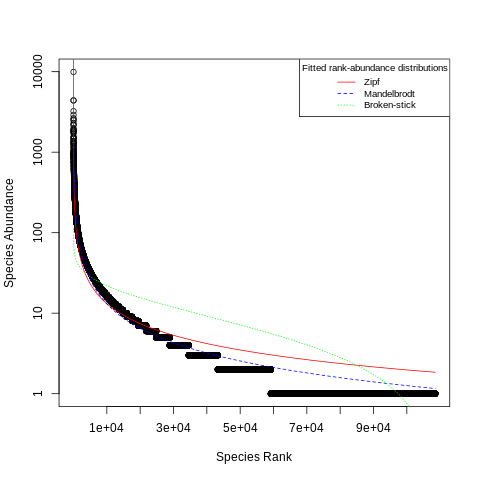
\includegraphics[width=\pfw]{figures/abundance_plot-twitter_200mio-view.png}}
  \subfigure[Distribution of the OSM dataset]{
    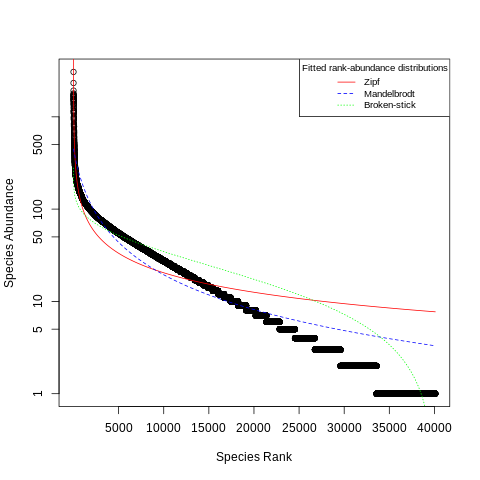
\includegraphics[width=\pfw]{figures/abundance_plot-asia_200mio-view.png}}
  \caption{Distributions of different datasets with fitted distribution curves}
  \label{fig:distris}
\end{figure}

To have a discussion of optimal configurations for CBF, obvious topics are the optimum number of hash functions $k$, the optimum size of the filter $m$ and the bit depth $b$ for each layer. For CGMs the complexity is multiplied by the number of Layers $L$ which need to be configured with a size $m_x$ and bit depth $b_x$.

To make an informed decision about these parameters one aspect that is important is the (assumed) distribution of the data to be encoded. One way this can be approached is by modeling the distribution, using a well-known distribution such as the Zipf distribution \cite{zipf1945meaning}, the Mandelbrot distribution \cite{mandelbrot1967distribution}, or the Broken-stick distribution \cite{baumiller1992broken}. Such distributions can be (partially) fit to a subset of the data, for example with machine learning techniques \cite{pradoml}.

As depicted in Figure \ref{fig:distris}, the aforementioned models definitely don't fit our discrete and finite data, but their behavior seem to be a good model of the real-world data.

Starting from an assumption of how many data items are going to be modeled, one can now start to search the configuration space as follows: one needs to introduce a first layer which will receive all of the data. That is, one can sample from the given distribution and perform or simulate the insertion. It is important to now extract the overflow data items which would go to the second layer.

If one chooses a small bit depth and a moderate filter size, most of the slots will overflow and it is clear that the data distribution of overflowed data will be very similar to the previous layer. Only a few very rare instances from the long tail might be absorbed.
If, however, one chooses a comparably large filter size or larger bit depths or a combination of both, only the very frequent data items will overflow and, hence, the higher layers will see discrete distributions.

The real behavior can be anything between. Still, the take away is (1) that an optimal configuration is not possible as one cannot derive the statistical properties of the output distributions of the layers in general, and (2) that the number of different data items in higher layers decreases such that, as a consequence, the uniform distribution assumption of the Bloom filter theory gets broken.


%\missingfigure[figwidth=6cm]{Abundance Plot}


%\begin{comment}
%\begin{figure*}[t]
%  \def\pfw{.2\textwidth}
%  \centering
%  \subfigure[placeholder]{    
\includegraphics[width=\pfw, page=1]{figures/histograms_Asia 200 mio.pdf}}
%  \subfigure[placeholder]{    
\includegraphics[width=\pfw, page=2]{figures/histograms_Asia 200 mio.pdf}}
%  \subfigure[placeholder]{    
\includegraphics[width=\pfw, page=5]{figures/histograms_Asia 200 mio.pdf}}
%  \subfigure[placeholder]{    
\includegraphics[width=\pfw, page=5]{figures/histograms_Asia 200 mio.pdf}}
%
%  \caption{Distributions and Resolutions}
%  \label{fig:distr_res}
%\end{figure*}
%\end{comment}
%

\section{Operations on Counting GloBiMaps}\label{operations-on-counting-globimaps}

Counting GloBiMaps can be interpreted as representation of pointclouds on grids, which themselves can be representations of various spatial structures. This section describes some meaningful operations for spatial databases and gives hints on their precision.
The compressed representation combined with the expressiveness of some
of these operations make it feasible to perform ad-hoc approximations of
certain spatial queries and to perform calculations on clients and edge
devices on the fly without ever needing to query for the uncompressed input data.
%This goes far beyond the use of Bloom filters as index structures and opens
%the door for a range of new optimizations.

\begin{enumerate}
  \item{\textbf{UNION Operation} creates a union CGM by adding two CGMs}
  \item{\textbf{INTERSECTION Operation with MERGE function} creates an intersection CGM by merging the overlapping points of two CGMs using a merge function}
  \item{\textbf{SUM Operation} calculates a sum of an area given by a list of hash values}
\end{enumerate}

\subsection{Union and Intersection}\label{union-and-intersection}

The Counting GloBiMaps structure as an extension of GloBiMaps and
therefore of BFs has several interesting properties, which
shall be discussed here. BFs as representations of sets can
perform operations that are familiar from set theory such as
intersections and unions. In a binary bloom filter these can be
expressed using a simple binary operation such as bitwise OR and bitwise
AND directly on the bloom filter data.

When using Counting Bloom Filters this is a bit less straight forward to
implement and for Counting GloBiMaps the layered structure needs to be
taken into account. Nonetheless, these operations can be quite useful for
various applications therefore algorithms for implementing these
operations will be presented along with an analysis of the algorithms
complexity.

We shall also note the special case of a Counting GloBiMap that has a binary filter as its first layer (equivalent to a bit size of 1) which can exploit the simplicity of the binary operations for the first layer as known from BFs and GloBiMaps \cite{werner2019globimaps}.
% which  constitutes a significant optimization.

To understand the following algorithms, the insert and get operations are defined first to aid notation.

\begin{itemize}
  \item{
        $\get(A, i)$ takes as input a CGM $A$ and a bin-index $i$, it retrieves the value from the bin indexed by $i$ , escalating and summing up the values of higher layers when it encounters threshold values concordant to the algorithm of the GET operation in Listing \ref{ls:get-operation} }
  \item{
        $\insertv(A, i, v)$ takes as input a CGM $A$ and a bin-index $i$ and a value $v$, it inserts the value into the CGM similarly to the PUT operation described in Listing \ref{ls:put-operation}, in this case avoiding the need to call the hash function as the bin index is given.}
\end{itemize}

\subsection{Union Operation}\label{union-operation}

One way to interpret Counting GloBiMaps is as a Vector of $n$
dimensions, with $n$ being size of the largest layer. With this
definition the Union of two CGMs is a simple vector addition with the
simplest implementation for a single layer 1 bit CGM being a bitwise OR
operation. The Union allows for merging two disparate datasets into one CGM.

\begin{algorithm}
  \SetAlgoLined
  \KwIn{ CGM $A = \{k, {b_{A,x}, m_{A,x}}\} $
    $B = \{k, {b_{B,x}, m_{B,x}}\} x \in 1\dots \Lambda $
    $ m_{A,1} \geq m_{B, 1}$}
  \KwResult{CGM $I$}
  \text{initialize $I$ with $0$}

  \ForEach{ $i \in 0 \dots m_{A, 1}$}{
    \If{$ \val(\mod(i, m_{B}), L_{B,1}) \neq 0 \, \textbf{OR} \, \val(i, L_{B,1}) \neq 0$}{
      $s \leftarrow \get(B,i) + \get(A,i)$

      $\insertv(I, i, s)$
    }
  }
  \KwResult{$I$}
  \caption{Union Operation}
  \label{ls:union}
\end{algorithm}

The worst case complexity of the Union operation is:
$$O(\Sigma_{l = 1..L}{m_l}) = O(L \overline{m_l}) \approx O(L m_1)$$


\subsection{Intersection Operation Family }\label{intersection-operation}

When lifting the Intersection Operation to CGMs we have the opportunity to introduce a family of operations, derived from the classical intersection, which for single bit BFs would be the bitwise AND. For CBFs it would be an elementwise minimum operation.
In our construct we extend the notion of the elementwise operation by introducing a merge function $\textbf{merge}(v_a,v_b)$ taking the the value of th the Operands elements as input thereby generalizing the idea, that is implicit in the intersection operation in order to arrive at a set of operations known from computer graphics.
%The intersection operation takes two CGMs and produces a result CGM using a merge function which takes as input the values of the intersecting bins. This is the analogue to the intersection operation known from BFs that can be implemented using bitwise AND. In addition to the Algorithm we present four different merge functions: min, add, subtract, difference and mask.

\begin{algorithm}
  \SetAlgoLined
  \KwIn{ CGM $A = \{k, {b_{A,x}, m_{A,x}}\} $
    $B = \{k, {b_{B,x}, m_{B,x}}\} x \in 1\dots \Lambda $
    $ m_{A,1} \geq m_{B, 1}$
    $ \textbf{merge}(v_a ,v_b)$}
  \KwResult{CGM $I$}
  \text{initialize $I$ with $0$}

  \ForEach{ $i \in 0 \dots m_{A, 1}$}{
  \If{$ \val(\mod(i, m_{B}), L_{B,1}) \neq 0 \, \textbf{AND} \, \val(i, L_{B,1}) \neq 0$}{
    $v \leftarrow \textbf{merge}(\get(B,i), \get(A,i))$

    $\insertv(I, i, v)$
    }
  }
  \KwResult{$I$}
  \caption{Intersection Operation Family with textbf{merge} function}
  \label{ls:intersection}
\end{algorithm}

The worst case complexity of the Intersection operation is:

$$O(\Sigma_{l = 1..L}{m_l}) = O(L \overline{m_l}) \approx O(L m_1)$$


In the context of the union information, different slot values need to be aggregated taking into account the current values in the same slots of two different CGMs. The usual approach would be to take the sum of the values of the counters. This mimics the behavior of a filter in which all elements from both CGMs have been inserted. As mentioned before it is also possible to define other merge functions, for example minimum, subtract, difference, and mask. Especially the non-symmetric mask operation is interesting as it models the subset of $A$ that overlaps with $B$. As $B$ can be a single layer, single-bit GloBiMap, we can use this operation to perform basic spatial statistics on the compressed data representations in a CGM with respect to a GloBiMap as described in Section \ref{spatial-statistics}.
In the following some possible merge functions are reviewed.
\begin{itemize}
  \item{$\textbf{minumim}(v_a, v_b) = \min(v_a, v_b)$ Minimum implements a classical intersection \ref{spatial-statistics}.}
  \item{$\textbf{mask}(v_a, v_b) = v_a$ subset of $A$ that overlaps with $B$ useful for spatial statistics as described in Section }
  \item{$\textbf{add}(v_a, v_b) = v_a + v_b$ Adds the values where a spatial intersection occurs. This is is useful for aggregating results of different mask operations}
  \item{$\textbf{subtract}(v_a, v_b) = \max(v_a - v_b, 0)$ Subtracts the values where a spatial intersection occurs. This is is also useful for aggregating results of different mask operations}
  \item{$\textbf{difference}(v_a, v_b) = |v_a - v_b|$ takes the absolute difference between values . This is is also useful for aggregating results of different mask operations, when subtract function would lead to zero result values}
\end{itemize}


% The subtraction and difference subtract one value from the other, while subtraction is zero in cases where $v_b > v_a$. The difference function on the other hand, is defined as the absolute value of the subtraction.
% $$\textbf{subtract}(v_a, v_b) = \max(v_a - v_b, 0)$$
% $$\textbf{difference}(v_a, v_b) = |v_a - v_b|$$
% Finally the mask operation is especially useful for getting only the subset of $A$, that overlaps with $B$, here $B$ can even be a single layer Binary GloBiMap.

% $$\textbf{mask}(v_a, v_b) = v_a$$

% It is clear that some the merge function could be applied in the union operation instead of a simple addition.


\subsection{Spatial Statistics}\label{spatial-statistics}
In many tasks on geometric data, one is interested in spatial summaries such as how many objects fall into a given polygon or what is the average temperature measured in a city. To query a CGM for the sum of points in a given area, one can use the GET Operation over a suitably rasterized geometric region. A sensible optimization of such an operation, especially if an area will be reused over time, is to cache the hash function values $h_1$ and $h_2$ for each point of the rasterized geometry. This leads us to the SUM Operation described in the Listing \ref{ls:sum-operation}

\begin{algorithm}[h!]
  \SetAlgoLined
  \KwIn{ CGM $A = \{k, {b_{A,x}, m_{A,x}}\} \space x \in 1\dots \Lambda $
    list of hash values $h_{j,y} \text{, } y \in \{1,2\}\text{, } j \in 0 \dots N$}
  \KwResult{$z$}
  $z \leftarrow 0$

  \ForEach{ $j \in 0 \dots N$}{

    $v_{min} \leftarrow \infty$

    \ForEach{ $i \in 0\dots k$}{
      $s \leftarrow 0$

      \ForEach{$x \in 1..\Lambda$}{
        $j \leftarrow mod(h_{j,1} + (i + 1) * h_{j,2}, m_x)$

        $v \leftarrow val(j, L_{A,x})$

        $s \leftarrow s + v$

        \If{$v < 2^{b_x}-1$ OR $v = 0$}{
          \textbf{break}
        }
      }

      $v_{min} \leftarrow \min(v_{min}, s)$
      \If{$v_{min} = 0$}{
        \textbf{break}
      }
    }

    $z \leftarrow s + v_min$
  }
  \KwResult{$z$}
  \caption{SUM Operation}
  \label{ls:sum-operation}
\end{algorithm}

Depending on the constraints of the hardware and the number of polygons to cache this may or may not be a feasible strategy.

Another possible optimization especially useful if there are many and overlapping polygons is to encode the polygons in single layer Binary GloBiMaps one for each polygon along with a bounding box covering the polygon bounds and caching the hash functions for the whole possible 2D space. Then the sum can be computed by first applying the Intersection Operation with mask merge function and in a second step performing the SUM operation, using the cached hash functions covering the bounding box. Such complex combinations of stages that share similarities with sprite graphics can be surprisingly powerful, but are beyond the scope of this paper.

% \missingfigure[figwidth=6cm]{polygons or intersections}
% \clearpage

\section{Multiresolution Counting GloBiMaps}\label{multiresolution}
Quite a few times, we have already remarked that something bad is happening to the distribution properties from layer to layer.
By truncating away the less frequent data instances layer by layer, the variability of the data in higher layers is decreasing and this can
lead to degeneracies, for example, when the hash functions are not getting sufficiently diverse input to surjectively cover and use the allocated slots.
We therefore suggest a new strategy of remapping indices between layers increasing the randomness from layer to layer to counter the inherent decrease of variability. Keeping the CGM layer structure, instead of remapping the indices that get propagated with a simple modulo operation a new remapping technique involving discretization of the coordinates at a higher resolution is introduced.


\begin{figure}[h!]
  \def\pfw{.45\textwidth}
  \includegraphics[width=\pfw, page=2]{figures/CGM_Layer_Schema.pdf}
  \caption{CGM Multi Resolution Setup}
  \label{fig:cgm_mrs_schema}
\end{figure}



Therefore the CGM definition is extended with a resolution for each layer.
To simplify the discussion, let us assume (without loss of generality), that all input coordinates are scaled into the range $[0,1]$. Then, the resolution can be given by an integer number $r_x$ defining the cell division index to be the the coordinate multiplied by this resolution coefficient rounded down to the nearest integer.

$$CGM = \{k, L_x = \{m_x, b_x, r_x\} \} \space x=1..\Lambda  $$

What happens in this setting is that coordinates that are mapped to the same cell in low resolution will be re-mapped at higher resolution hoping that they might lead to different high-resolution coordinates and therefore, increased variability in the subsequent layer.
Depending on how the resolutions are used, one can generate a quadtree like refinement structure such that the first layers of such Counting GloBiMaps can be of rather low resolution expecting that they will be subdivided as soon as they get visited often enough thereby becoming more interesting. However, such an approach differs significantly from common raster data management as the subdivision occurs locally only.

In the following we will describe the modified PUT and GET operations.


\begin{algorithm}[h!]
  \SetAlgoLined
  \KwIn{ CGM $A = \{k, \{b_x, m_x, r_x\}\} \space x \in 1\dots \Lambda $

    Coordinate $c$ }
  $c_{1}  \leftarrow c \cdot r_1$

  $h_1, h_2 \leftarrow \hash(c_{r_1}) $

  \ForEach{ $i \in 1\dots k$}{
    \ForEach{ $x \in 1 \dots \Lambda$}{
      \If{$x > 1$}{
        $c_{x}  \leftarrow c \cdot r_x$
      }
      $j \leftarrow \mod(h_1 c_{x, 1} + i h_2 c_{x, 2}, m_x)$

      $v \leftarrow \val(j, L_{A,x})$

      \If{$v < 2^{b_x}-1$}{
        $\val(j, L_{A,x}) \leftarrow v + 1$

        \textbf{break}
      }
    }
  }
  \caption{Multiresolution PUT Operation}\label{ls:mrs-put-operation}
\end{algorithm}


The multiresolution PUT operation described in Listing \ref{ls:mrs-put-operation} is similar in structure to the PUT Operation described in Listing \ref{ls:put-operation}, but with the addition of calculating the resolution for each layer that is is visited. Note that we can use the hashing trick and add the rasterized coordinate values as factors for $h_1$ and $h_2$.
Alternatively, one can calculate new hash values for each layer.

The multiresolution GET operation comes in a few different flavors which are necessary due to the fact, that the number of layers affected by a given coordinate is not predictable and therefore the resolution at which the data is held in practice is not known beforehand. Therefore we suggest to either query for a specific resolution layer in which case there are two possible outcomes: either the coordinate exists in the given resolution, which means it can be returned or it does not in which case the GET operation can either return a special state, such as $-1$ or it can return the the highest resolution value below the queried resolution.
The other option is to query without asking for a specific resolution in which case there are two possible result strategies: either the operation returns the highest resolution it can find and returns it along with the resolution value. The other option is to return all found resolutions and return them along with the values in a container such as a list, array or hashmap.



\begin{algorithm}
  \SetAlgoLined
  \KwIn{ CGM $A = \{k, {b_x, m_x, r_x}\} \space x \in 1\dots \Lambda $

    Coordinate $c$}
  \KwResult{$v_{min}$
    $r_v$
  }
  $c_{1}  \leftarrow c * r_1$

  $h_1, h_2 \leftarrow \hash(c_1)$

  $v_{min} \leftarrow \infty$

  \ForEach{ $i \in 0\dots k$}{
    $s \leftarrow 0$
    $r_t \leftarrow 0$

    \ForEach{$x \in 1..\Lambda$}{
      \If{$x > 1$}{
        $c_{x}  \leftarrow c * r_x$
      }
      $j \leftarrow \mod(h_1 c_{x, 1} + i h_2 c_{x, 2}, m_x)$

      $s \leftarrow s + \val(j, L_{A,x})$

      $r_t \leftarrow r_x$

      \If{$\val(j, L_{A,x}) = 0$}{
        \KwResult{$0$, $r_1$}
      }
      \If{$\val(j, L_{A,x}) < 2^{b_x}-1$}{
        \textbf{break}
      }
    }
    $v_{min} \leftarrow \min(v_{min}, s)$
    \If{$s = v_{min}$}{
      $ r_v \leftarrow r_t$
    }
  }
  \KwResult{$v_{min}$, $r_v$}
  \caption{Multiresolution GET Operation returning highest resolution}
  \label{ls:mrs-get-operation_highest}
\end{algorithm}


\begin{algorithm}
  \SetAlgoLined
  \KwIn{ CGM $A = \{k, {b_x, m_x, r_x}\} \space x \in 1\dots \Lambda $

    Coordinate $c$}
  layer $x$
  \KwResult{$v_{min}$
  }
  $c_{1}  \leftarrow c * r_1$

  $h_1, h_2 \leftarrow \hash(c_1)$

  $v_{min} \leftarrow \infty$

  \ForEach{ $i \in 0\dots k$}{
    $s \leftarrow 0$

    \If{$x > 1$}{
      $c_{x}  \leftarrow c * r_x$
    }
    $j \leftarrow \mod(h_1 c_{x, 1} + i h_2 c_{x, 2}, m_x)$

    $s \leftarrow s + \val(j, L_{A,x})$

    $r_t \leftarrow r_x$

    \If{$\val(j, L_{A,x}) = 0$}{
      \KwResult{$0$, $r_1$}
    }

    $v_{min} \leftarrow \min(v_{min}, s)$
  }
  $v_{min} \leftarrow v_{min} + \Sigma_{i=1}^{x}{t_i}$

  \KwResult{$v_{min}$}
  \caption{Multiresolution GET Operation with resolution query}
  \label{ls:mrs-get-operation_resq}
\end{algorithm}


% \vfill\null


\begin{figure*}[t]
  \def\pfw{.24\textwidth}
  \centering
  \subfigure[Scatterplot for the first 100 mio points of the Twitter dataset]{
    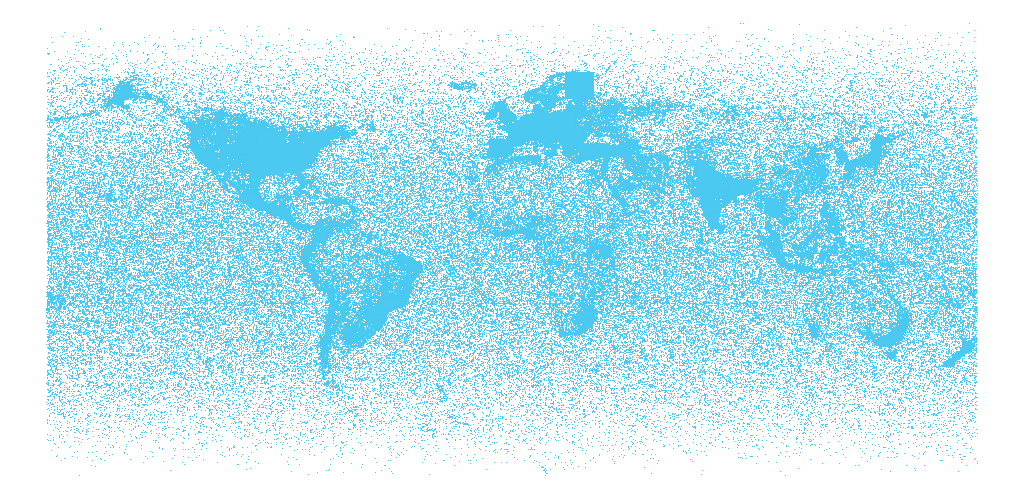
\includegraphics[width=\pfw]{figures/rtwitter_coords_plot.png}}
  \subfigure[Scatterplot for the first 100 mio points of the OSM dataset]{
    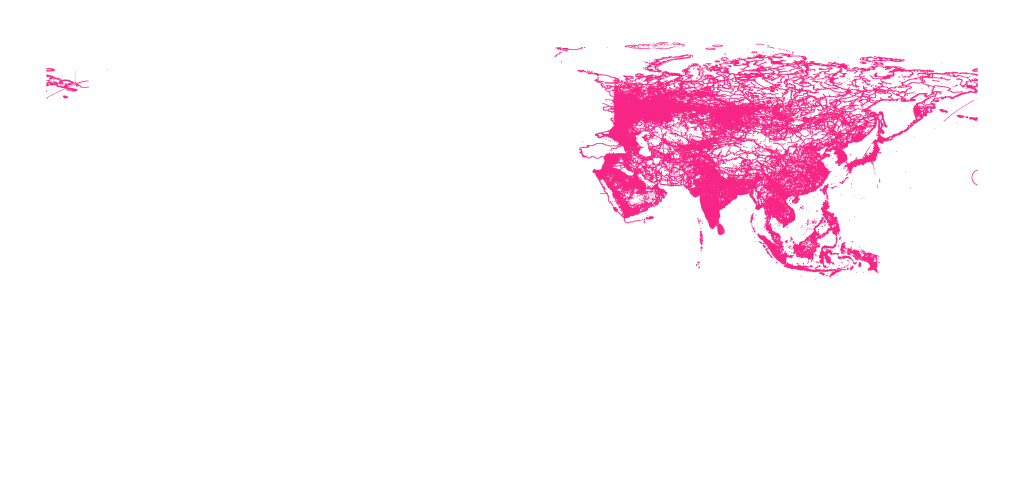
\includegraphics[width=\pfw]{figures/rasia-latest_plot.png}}
  % \caption{Pointcloud Datasets}
  % \def\pfw{.48\textwidth}
  % \centering
  \subfigure[US Census Zip Codes]{
    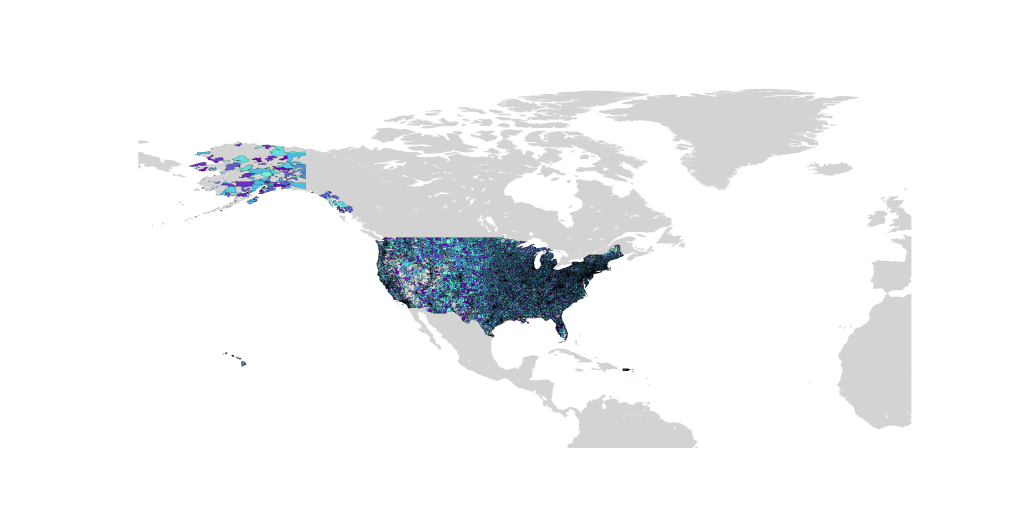
\includegraphics[width=\pfw]{figures/rtl_2017_us_zcta510_bb.png}}
  \subfigure[Global Administrative Boundaries]{
    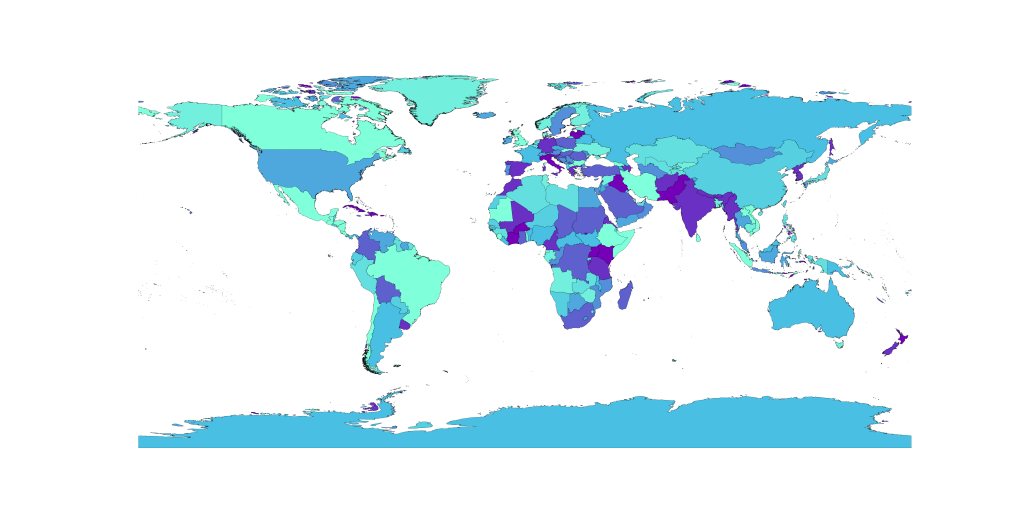
\includegraphics[width=\pfw]{figures/rGlobal_LSIB_Polygons_Detailed.png}}
  \caption{Pointcloud and vector datasets}
  \label{fig:pointclouds}
  \label{fig:vectors}
\end{figure*}

%\vfill\null
\section{Evaluation}\label{evaluation}

This section shall describe the experiments that were performed in order to show the properties of CGM on datasets related to human activity on Earth. Because of the big amount of configurable parameters, e.g.amounts, sizes and bit-depth of layers, number of hash functions and different resolutions of the dataset discretizations, the experiments are structured in such a way as to attempt to isolate the behavior of each parameter.
%Additionally an attempt is made to come up with a recipe for optimizing these parameters given enough information on the to be encoded data in order to keep the loss of precision acceptable.

\begin{table*}[b!]
  \centering
  \begin{tabular}{|c|c|l|c|c|c|}
    \hline
    \multirow{2}{*}{\bfseries Dataset}   &
    \multirow{2}{*}{\bfseries Size}      &
    \multirow{2}{*}{\bfseries Optimal k} &
    \multicolumn{3}{|c|}{\bfseries Encoding time}                                                                                                      \\
    \cline{4-6}                          &                      &   & min                                                        & max         & mean  \\
    \hline
    Twitter                              & 213,869,519 points   & 3 & 10.0824                                                    & 16.0112     & 13.87 \\
    \hline
    OSM                                  & 1,563,146,114 points & 6 & 73.1999                                                    & 98.5461     & 88.07 \\
    \hline
                                         &                      &   & \multicolumn{3}{|c|}{\bfseries \# of pixels @ 16384x16384}                       \\
    \hline
    Global Administrative Boundaries     & 4456 polygons        & - & 0                                                          & 4.95708e+07 & 39849 \\
    \hline
    Us Census Zip Codes                  & 43,431 polygons      & - & 0                                                          & 61710
                                         & 161.876                                                                                                     \\
    \hline
  \end{tabular}
  \caption{Properties of datasets}
  \label{tab:datasets}
\end{table*}


\subsection{Datasets}\label{datasets}

Two pointcloud datasets were used in this experiment; the first is a collection of twitter locations and the second is a collection of Open Street Maps(OSM) point objects. With respect to the spatial statistics queries, polygon datasets of US zip codes as well as bounding polygons of all countries in the world have been used.
Table \ref{tab:datasets} gives some characteristics of these datasets.

\begin{figure*}[t]
  \def\pfw{.245\textwidth}
  \centering

  \subfigure[Twitter error rate for values of k]{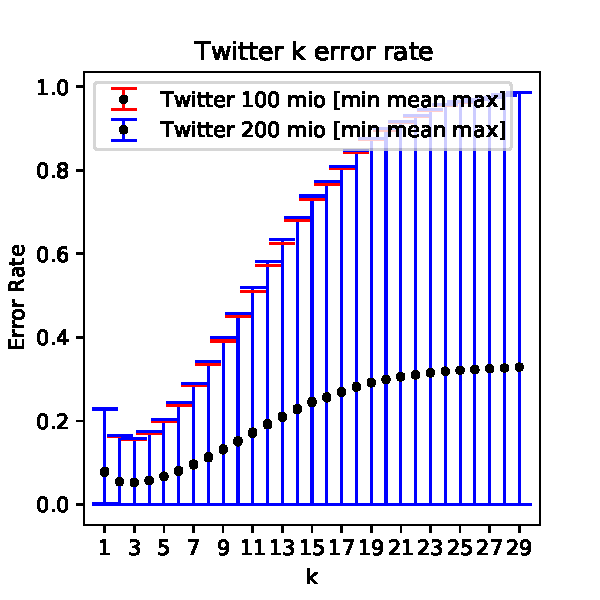
\includegraphics[width=\pfw, page=1]{figures/test_datasets_for_k_matrices_clean.pdf}}
  \subfigure[OSM error rate for values of k ]{\includegraphics[width=\pfw, page=2]{figures/test_datasets_for_k_matrices_clean.pdf}}
  \subfigure[Twitter distribution of bin sizes ]{\includegraphics[width=\pfw, page=2]{figures/resolutions2_histograms.pdf}}
  \subfigure[OSM distribution of bin sizes]{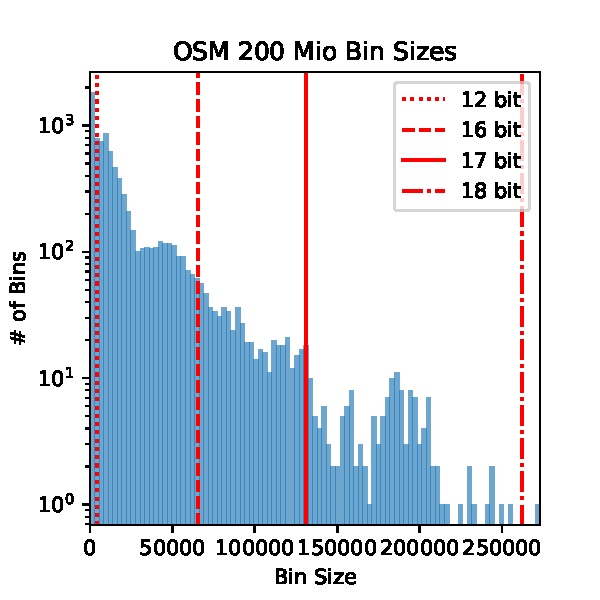
\includegraphics[width=\pfw, page=1]{figures/resolutions2_histograms.pdf}}
  \caption{Pointcloud Dataset Properties}
  \label{fig:error_rate_resolutions}
\end{figure*}



\subsubsection{Global Twitter Dataset}\label{twitter-dataset}
The Twitter dataset consist of more than 270 million individual locations mined from Twitter.
This dataset shows usage patterns with highest densities in North america and Europe \cite{werner2019globimaps}.
It also features a certain percentage of random locations which are distributed across the globe, due to bot activity. This dataset has been subdivided by taking the first $N$ points for values of 1 million, 10 million, 50 million, 100 million, and 200 million. Except for scaling and discretization which was applied in the following experiments in order to encode the dataset into a CGM, no further processing or data cleaning was applied.




\subsubsection{OpenStreetMap (OSM) Dataset}\label{osm-asia-dataset}
OpenStreetMap is an editable map database built and maintained by volunteers \cite{OpenStreetMap}.
In \ref{fig:pointclouds} the OSM dataset is depicted, which is a collection of points derived from OSM data. It consists of more than $1.5$ billion points that are located on the Asian continent. This dataset has been subdivided by taking the first $N$ points for values of 200 million, 500 million and 1 billion. Except for scaling and discretization which was applied in the following experiments no further processing or cleaning was applied.

% \vfill\null


\subsubsection{Polygon Dataset US Census Zip Codes}
The US census dataset consists of 2017 Census Zip Codes Polygons, which are all in all more than 44 thousand individual polygons of various sizes.
They cover the area of the United States, with higher density of polygons around more densely populated areas, which correlates with areas of higher density in the Twitter dataset.
The dataset was downloaded from the United States Census Bureau website in the form of shapefiles. Apart from scaling and rasterization in various resolutions, no further processing was applied.
\cite{bureau_tiger/line_nodate}

\subsubsection{Global LSIB Polygons Detailed}
The LSIB Polygons Dataset has been downloaded in shapefile format from the Humanitarian Data Exchange. it consists of more than 4000 highly detailed polygons and  is described as follows:

\textquote{
  The Office of the Geographer’s Global Large Scale International Boundary Detailed Polygons file combines two datasets, the Office of the Geographer’s Large Scale International Boundary Lines and NGA shoreline data. The LSIB is believed to be the most accurate worldwide (non- W. Europe) international boundary vector line file available.
}
\cite{noauthor_global_nodate}
Other than scaling and rasterization in various resolutions, no further processing was applied.



\begin{figure*}[ht!]
  \def\pfw{.23\textwidth}
  \centering
  \subfigure[Error Sizes for Different Datasets]{ 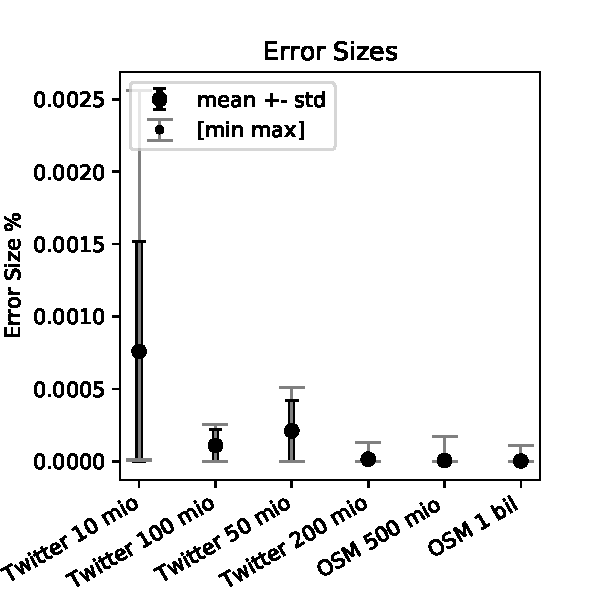
\includegraphics[width=\pfw, page=1]{figures/test_datasets_with_errord_ds.pdf}}\label{subfig:test_datasets_with_errord_ds}
  \subfigure[Error Sizes for Different Sizes of the Data Structure]{ 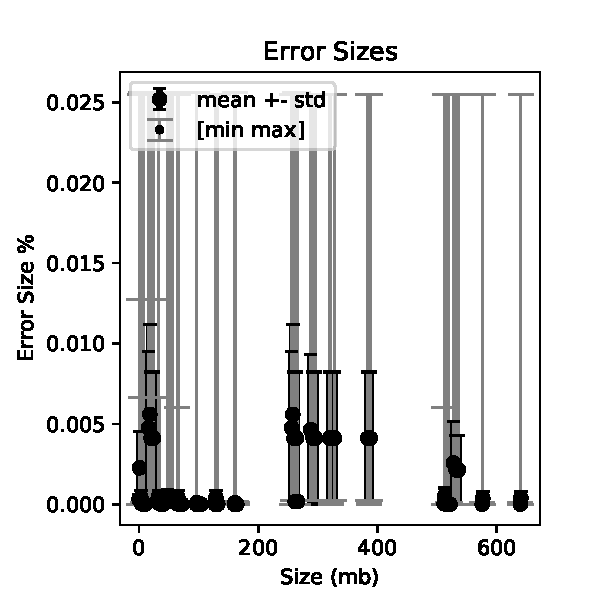
\includegraphics[width=\pfw, page=1]{figures/test_datasets_with_errord_sizes.pdf}}\label{subfig:test_datasets_with_errord_sizes}
  \subfigure[Error Sizes for Compression Ratios lower value means more Compression]{ 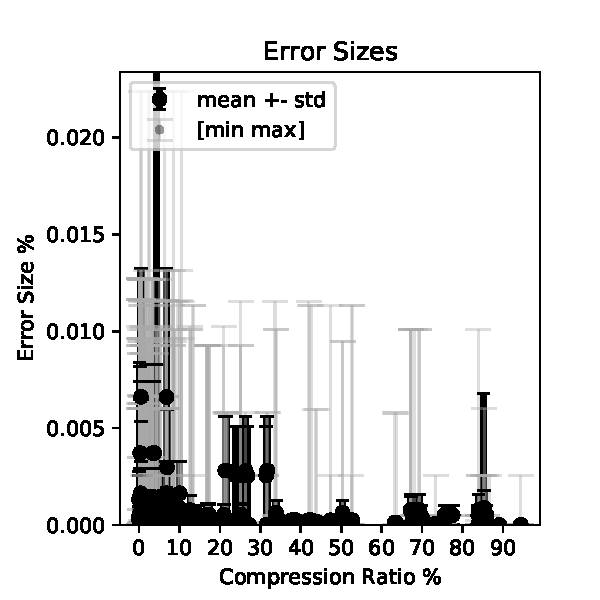
\includegraphics[width=\pfw, page=1]{figures/test_datasets_with_errord_compression.pdf}}\label{subfig:test_datasets_with_errord_compression}
  \subfigure[Error Sizes for different Compression Ratios]{ \includegraphics[width=\pfw, page=2]{figures/test_datasets_with_errord_compression.pdf}}\label{subfig:test_datasets_with_errord_compression2}

  \caption{Error Sizes are in Relation to the Size of the dataset}
  \label{fig:error_size}
\end{figure*}

\subsection{Analyzing the Importance of Resolutions}
When deciding on a resolution in which to rasterize points for the inclusion in Counting GloBiMaps, several aspects can be of importance. First the resolution will decide the actual spatial accuracy of points added to the data structure, which is highly application dependent and will not be discussed here. Beyond that, various properties that change given a different resolution, such as unique number of points and bin size distributions, that have an impact on fraction of zeros $\foz$ and expected error size as shown earlier. Table \ref{table:Resolutions} presents an overview.

\begin{table*}[b!]
  \centering
  \begin{tabular}{|c|c|l|c|c|c|c|c|}
    \hline
    \multirow{2}{*}{\bfseries Dataset}       &
    \multirow{2}{*}{\bfseries Resolution}    &
    \multirow{2}{*}{\bfseries Unique points} &
    \multicolumn{5}{|c|}{\bfseries Bin Size}                                                                               \\
    \cline{4-8}                              &        &           & mean & max        & 25th \%ile & e Median & 75th \%ile \\
    \hline
    OSM 200 Mio                              & 4,096  & 677,700   & 295  & 241,790    & 6          & 26       & 103        \\
    \hline
    OSM 200 Mio                              & 8,192  & 1,738,582 & 115  & 96,161     & 3          & 12       & 46         \\
    \hline
    OSM 200 Mio                              & 16,384 & 4,156,942 & 48   & 32,540     & 2          & 7        & 23         \\
    \hline
    OSM 200 Mio                              & 32,768 & 9,311,414 & 21   & 13,072     & 2          & 4        & 13         \\
    \hline
    Twitter 200 Mio                          & 4,096  & 1,409,058 & 142  & 17,020,560 & 1          & 1        & 3          \\
    \hline
    Twitter 200 Mio                          & 8,192  & 1,983,080 & 100  & 16,769,560 & 1          & 1        & 5          \\
    \hline
    Twitter 200 Mio                          & 16,384 & 2,845,933 & 70   & 15,801,333 & 1          & 1        & 5          \\
    \hline
    Twitter 200 Mio                          & 32,768 & 3,987,981 & 50   & 15,769,401 & 1          & 1        & 6          \\
    \hline
  \end{tabular}
  \caption{Resolution properties}
  \label{table:Resolutions}
\end{table*}

Looking at the Table \ref{table:Resolutions}, we can clearly see that the two datasets with same number of points have wildly different properties, whereas the OSM dataset at a resolution of $16,384$ already has a maximum bin size smaller than $2^{15}$ and can therefore be fully represented with bit-depths of $15$ bits and smaller. The Twitter dataset at the same resolution has a minimum bit-depth of $24$ bits but the number of unique points is not even half the amount in comparison. Interestingly the the median and 75th percentile for the Twitter dataset are much lower, which leads to the conclusion that the Twitter dataset has a few highly concentrated hotspot, whereas the OSM dataset has a more even distribution, which is confirmed by Figures \ref{fig:error_rate_resolutions}. In such a case the multilayer architecture of CGMS can be exploited by adding a layer with a high bit-depth $b_x$ relatively small filter size $m_x$ at the top of the layer stack.


\subsection{Error Rate Distribution for Different Values of k}
\label{error-rate-distribution-for-different-values-of-k}
In order to analyze the optimum number of hash functions $k$ for a given dataset, a search over all values for $k$ between $1$ and $30$ was performed.
The CGMs have been configured with a range of configurations using bit-depth values of $1$, $8$, $16$ and $32$ bits and layers sizes of $2^{16}$, $2^{20}$,$2^{24}$ slots with layer counts $\Lambda$ between 1 and 3, and the datasets were rasterized to a resolution of $8192*8192$ pixels.
Measuring the representation quality of a Counting GloBiMaps was done by taking the fraction of the erroneous pixels divided by the number of pixels that are greater than zero, this is called the error rate:

$$ERR = \frac{\text{\# Erroneous Pixels}}{\text{\# Pixels > 0}}$$

In order to verify the ideal number of hash functions $k$ the error rate was calculated and plotted.
As seen in Figures \ref{fig:error_rate_resolutions}, the ideal number of $k$, that is the $k$ with the lowest error rate achieved, is different for the two datasets.
%\begin{comment}
%The ratio of uinque pixels $n$ and total number of point $t$ is important in this context.
%* OSM 200 mio with resolution $8192*8192$ pixels $n= 1738582, t= 200000000 $ $\frac{t}{n} = 115.0$
%* Twitter 200 mio with resolution $8192*8192$ pixels $n= 1983080, t= 200000000 $ $\frac{t}{n} = 100.8$
%
%\end{comment}
%


\subsection{Magnitudes of Errors}

To investigate the magnitude of errors, the datasets were encoded into the data structure as well as into a hashmap with a key for every point in the grid using a resolution of $8192*192$ pixels.
The CGMs have been configured with a range of configurations using bit-depth values $b_x$ of $1$, $8$, $16$ and $32$ bits and layers sizes $m_x$ of $2^{16}$, $2^{20}$,$2^{24}$ with layer counts $\Lambda$ between 1 and 3 and a number of hash function $k=8$.
After the encoding process, for each point on the grid the difference was taken between the encoded value and the correct value in the hashmap.
From this min, max, mean and histogram values were taken, which subsequently have been used to calculate the min, max, mean and std values seen in Figures \ref{fig:error_size}.

Figure \ref{fig:error_size} $a)$ shows a comparison of error size for different sized datasets, the error sizes here have been normalized to the number of points in the dataset, whereas configurations that can't hold the largest bin sizes or have a compression ratio $\text{cr} > 1.0$ where omitted.
It is shown that bigger datasets have a smaller relative error which is due to the fact that error size does not scale linearly with the number of points.

Figure \ref{fig:error_size} $b)$ shows a comparison of error size for different sized CGMs, the error sizes here have been normalized to the number of points in the dataset, whereas configurations that can't hold the largest bin sizes are bigger than $1$ gb or have a compression ratio $\text{cr} > 1.0$ where omitted.
It is clear, that bigger CGMs tend to have smaller error sizes, which is due to compression ratios which are highlighted in Figure \ref{fig:error_size} $c)$ and $d)$, showing error size on the y-axis and the compression ratio on the x-axis. To calculate the the compression ratios the number of bytes of the filters in the CGMs was divided by the number of points in the dataset times 8, presuming 64 bit or 4 bytes for each element of the coordinate.


\subsection{Performance Metrics}

\begin{figure*}[ht!]
  \def\pfw{.3215\textwidth}
  \centering
  \subfigure[Data Structure Insertion Performance for Different Sizes of Datasets]{    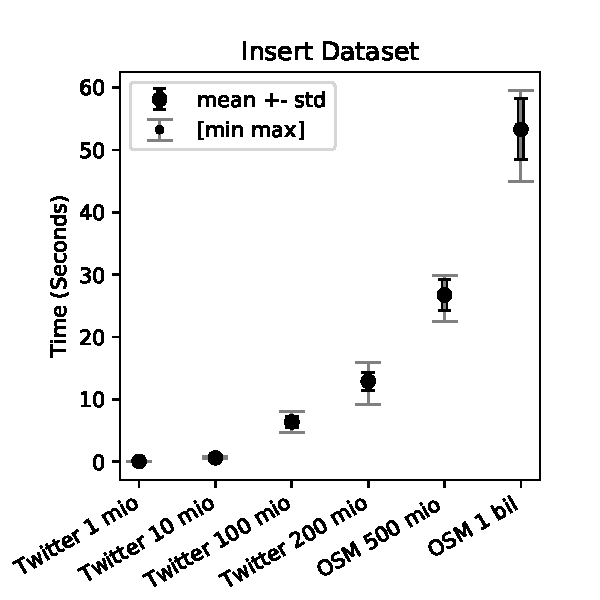
\includegraphics[width=\pfw, page=1]{figures/test_datasets_new_ds_size.pdf}}\label{subfig:insert_ds_size}
  \subfigure[Query performance for different sizes of datasets (Time for querying 100 mio points)]{    \includegraphics[width=\pfw, page=2]{figures/test_datasets_new_ds_size.pdf}}\label{subfig:query_ds_size}
  \subfigure[Query performance for different sizes of data structures (Time for querying 100 mio points) ]{    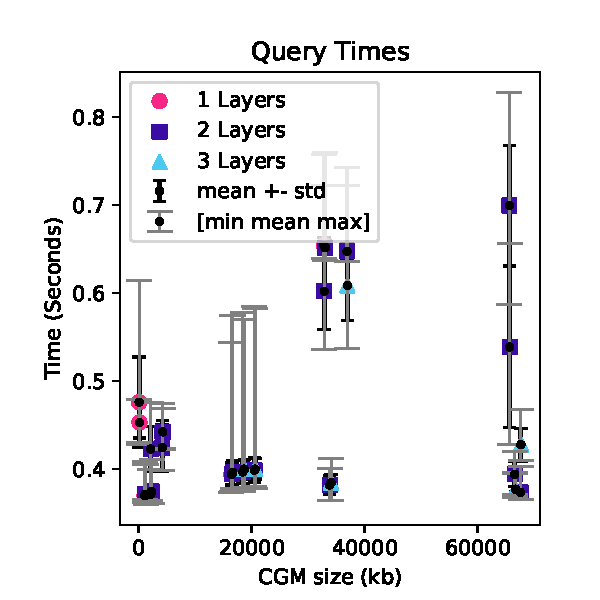
\includegraphics[width=\pfw, page=1]{figures/test_datasets_new_plot.pdf}}\label{subfig:query_filter_size}

  \caption{Performance}
  \label{fig:performance}
\end{figure*}

The evaluation of the performance of the data structure in terms of wall-clock time was performed using a clean and simple C++ implementation running on a common 64 bit system. No micro-optimizations have been done, which leads to some variance in the performance as can be seen in the figures. Overall, we can conclude that the performance of this initial implementation is adequate.


To evaluate the performance of the data structure, insertion of datasets of different sizes was measured for a selection of different configurations. For all tests a grid size of $8096*8096$ pixels was used.
The CGMs were configured with a range of configurations using bit-depth values $b_x$ of $1$, $8$, $16$ and $32$ bits and layers sizes $m_x$ of $2^{16}$, $2^{20}$ and $2^{24}$ with layer counts $\Lambda$ between 1 and 3 and a number of hash function $k=8$.

In a second step, the encoded data structures where queried with a workload of 100 mio uniform randomly distributed points within the grid size. This was done 10 times to generate a minimum, maximum and mean query time.

In figure \ref{fig:performance} $a)$ The linear scaling for inserting the data into the data structure is visible. This is not surprising as insertion of a single pixel is in theory dependant size of layers and to so extend the number of layers, this might be apart from noise caused by the operating system and other processes, what is responsible for the scaling of the standard deviation and the min and max values.

In figure \ref{fig:performance} $b)$ the time to perform the workload is shown for different sizes of encoded datasets. It is clear that the size of the dataset has no measurable impact, even though some of the queries will stop earlier in less populated structures created by smaller datasets, due to never reaching the upper layers. Other factors are more important here. As only layer numbers from 1 till 3 have been evaluated here, higher layer counts might change this statistic, although higher numbers of layers are not suggested as a strategy.

In figure \ref{fig:performance} $c)$ the time to perform the workload is shown for different sizes of CGMs a scaling law is not as clearly identifiable here. Although the slowest times tend to dominate on the right side with bigger CGMs, neither the size nor the number of layers seem to be a good predictor. Further investigation might be necessary as this could be heavily dependant on the implementation and properties of the hardware. Factors such as page swapping branch prediction and cache misses might play a role here as well as other properties of the filter that have not been investigated at this point.

% \todo{more text?}



\subsection{Error for Point in Polygon Counts}
\label{error-for-point-in-polygon-counts}

As mention previously, there are two ways that point in polygon counts can be achieved, the first is using the points of the rasterized polygon and queries the CGM for each point, this can be optimized by precalculating the hash functions for each point. The second way is encoding the rasterized polygon points into a single layer Binary CGM and using the previously described algorithm to calculate the sum. In both cases we can calculate the error for each polygon by taking the difference of the real sum $sum{real}$ and the sum containing errors
$sum_{err}$ and dividing it by the real sum.

$$PERR = \frac{|sum_{real} - sum_{err}|}{sum_{real }}$$

Summarizing the errors over all polygons, an error distribution is constructed and evaluated.

In this experiment, the polygons and pointclouds have been rasterized at a resolution of $16384*16384$ pixels. The pointclouds used where the first 1 mio and first 10 mio coordinates of the Twitter dataset. The CGMS where configured with a range of configurations using bit-depth values $b_x$ of $8$, $16$ and $32$ bits and layers sizes $m_x$ of $2^{16}$, $2^{20}$ and $2^{24}$ with layer counts $\Lambda$ between 1 and 3 and a number of hash function $k=8$.

Subsets of the Twitter dataset in the sizes 1 mio, 10 mio and 100 mio, were used to evaluate both polygon datasets.

In Figure \ref{fig:pip} $a)$ and $b)$ the performance of both polygon dataset across different point cloud sizes is plotted.

Figure \ref{fig:pip} $c)$ the performance of the US Zip Codes dataset is further investigated in relation to the bit-depth of the last showing that higher bit-depths in the last filter lead to smaller error sizes.

Furthermore in Figure \ref{fig:pip} $c)$ the impact of compression on error size for the US Zip Codes dataset is displayed. Showing that strong compression does not necessarily mean higher error size, although the likelihood of big errors seems to go down with lower compression.

%Notable here is the difference in performance between the US Zip Codes dataset and the Global Administrative Boundaries dataset, with the latter performing much worse, with a large deviation. The reasons for this behavior are not fully explained by the current experiments. But one obvious difference between the two datasets is the relative size of polygons which is much smaller for the zip code areas and the geographic positioning, with the US having the highest density of tweets.



\begin{figure*}[t!]
  \def\pfw{.24\textwidth}
  \centering
  \subfigure[Polygon sum error for US Zip codes]{    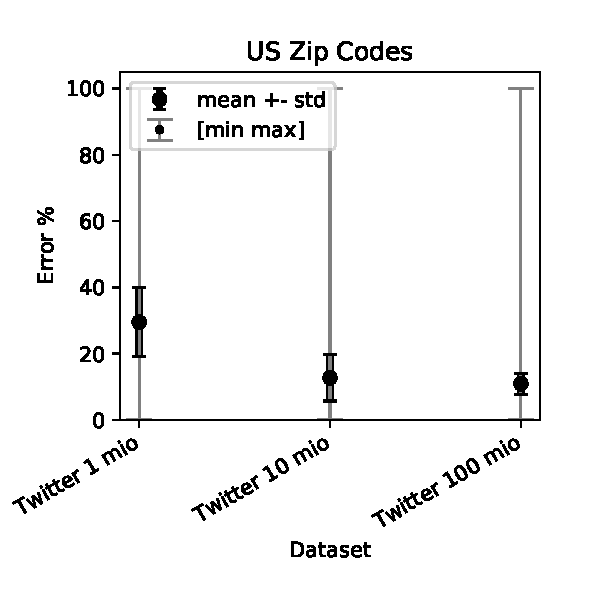
\includegraphics[width=\pfw, page=1]{figures/polygons_mask_plot.pdf}}
  \subfigure[Polygon sum error for Global Administrative Boundaries]{    \includegraphics[width=\pfw, page=6]{figures/polygons_mask_plot.pdf}}
  \subfigure[Polygon sum error for bit-depths of last filter]{    \includegraphics[width=\pfw, page=3]{figures/polygons_mask_ff.pdf}}
  \subfigure[Polygon sum error for compression ratios]{    \includegraphics[width=\pfw, page=5]{figures/polygons_mask_comp.pdf}}

  \caption{Point in Polygon Error Resistance}
  \label{fig:pip}
\end{figure*}

% \subsection{Optimal Parameter Selection}
% As has been shown selecting optimal parameters for known dataset is not trivial but can be achieved. For unknown datasets a prediction of distribution might be useful as well as an understanding upper bounds bin sizes in order to configure bit depths of layers.

%\subsection{Optimal Parameter Selection}
%\blindtext[2]

% \vfill\null

\section{Conclusions}\label{conclusion}
\balance
In this paper, we have introduced Counting GloBiMaps as a novel data structure to deal with large datasets of events or point clouds. It extends on previous work on GloBiMaps in that it first introduces small counters as in the Counting Bloom Filter paradigm and then a layered structure to accommodate counter overflows. To counter the reducing randomness of hash value distributions, we introduce a concept based on increasing the resolution to disambiguate ambiguous cells in later layers. Combined with a small jitter on the input data (unless there is natural noise like in GPS datasets), this provides a versatile and powerful randomized data modeling scheme from its functionality somewhere between frequency count rasters and point clouds. We show that set operations such as Union and Intersection can be lifted from Bloom filters with some work and that even counting queries over complex geometries such as polygons can be efficiently computed. A series of experiments shows that the data structure is practicable and efficient for the tasks it was designed for.

% \begin{acks}
%   This work was supported by the [...] Research Fund of [...] (Number [...]). Additional funding was provided by [...] and [...]. We also thank [...] for contributing [...].
% \end{acks}


% \clearpage
\balance
\bibliographystyle{ACM-Reference-Format}
\bibliography{cite}


\end{document}
\endinput
